\fenicschapter{Automatic calibration of depositional models}
              {Automatic calibration of depositional models}
              {Hans Joachim Schroll}
              {schroll}

A novel concept for calibrating depositional models is presented.  In
this approach transport coefficients are determined from well output
measurements.  Finite element implementation of the multi-lithology
models and their duals is automated by the FEniCS project DOLFIN using
a Python interface.

%\index{important term}

%------------------------------------------------------------------------------
\section{Issues in sedimentary deposition}

Evidence indicates that millions of years of pressure cooking
transforms the remains of living organisms into crude oil and natural
gas.  This process takes place in sealed reservoirs, so-called
structural and/or stratigraphic traps in the reservoir rock.  To
identify potential new reservoirs, it is of great interest to
understand the geological evolution of depositional basins in the
Earth's crust.  Different types of forward computer models are used by
sedimentologists and geomorphologists to simulate the process of
sedimentary deposition over geological time periods.  The models can
be used to predict the presence of reservoir rocks and stratigraphic
traps at a variety of scales. State-of-the-art advanced numerical
software, like for example DIONISOS by Beicip-Franlab, provides
accurate approximations to the mathematical model, which commonly is
expressed in terms of a nonlinear diffusion dominated PDE system.  The
potential of today's simulation software in industrial applications is
limited however, due to major uncertainties in crucial material
parameters that combine a number of physical phenomena and therefore
are difficult to quantify.  Examples of such parameters are diffusive
transport coefficients.

The idea in this contribution is to calibrate uncertain transport
coefficients to direct observable data, like well measurements from a
specific basin.  In this approach the forward evolution process,
mapping data to observations, is reversed to determine the data; that
is, transport coefficients.  Mathematical tools and numerical
algorithms are applied to automatically calibrate geological models to
actual observations --- a critical but so far missing link in forward
depositional modeling.

Automatic calibration, in combination with stochastic modeling, will
boost the applicability and impact of modern numerical simulations in
industrial applications.

%------------------------------------------------------------------------------
\section{A multidimensional sedimentation model}

Submarine sedimentation is an evolution process.  By flow into the
basin, sediments build up and evolve in time.  In dual lithology
models two types of sediments are considered, sand and mud.  The
evolution follows geophysical laws, expressed as diffusive PDE models.
The following system is a multidimensional version of the model
by~\citet{Rivenaes1992, Rivenaes1993}:
\begin{equation} \label{eq:schroll:model}
\left(\begin{array}{rl} A & s \\ -A & 1-s \end{array}\right)
\left(\begin{array}{c} s \\ h \end{array}\right)_t =
\nabla \cdot \left( \begin{array}{l} \alpha s \nabla h \\ \beta (1-s) \nabla h \end{array} \right)
\enspace \hbox{in} \enspace [0,T] \times B.
\end{equation}
Here $h$ denotes the thickness of a layer of deposit and $s$ models
the volume fraction for the sand lithology.  Consequently, $1-s$ is
the fraction for mud.  The system is driven by fluxes anti
proportional to the flow rates $s \nabla h$ and $(1-s) \nabla h$
resulting in a diffusive, but incompletely parabolic, PDE system.  The
domain of the basin is denoted by $B$.  Parameters in the model are:
The transport layer thickness $A$ and the diffusive transport
coefficients $\alpha$, $\beta$.

For a forward in time simulation, the system requires initial and
boundary data.  At initial time, the volume fraction $s$ and the layer
thickness $h$ need to be specified. According to geologists, such
data can be reconstructed by some kind of ``back stripping''.  Along
the boundary of the basin, the flow rates $s \nabla h$ and
$(1-s) \nabla h$ are given.

%------------------------------------------------------------------------------
\section{An inverse approach}

The parameter-to-observation mapping $R: (\alpha, \beta) \mapsto (s,
h)$ is commonly referred to as the forward problem.  In a basin direct
observations are only available at wells. Moreover, from the age of
the sediments, their history can be reconstructed.  Finally, well-data
is available in certain well areas $W \subset B$ and backward in time.

The objective of the present investigation is to determine transport
coefficients from observed well-data and in that way, to calibrate the
model to the data. This essentially means to invert the
parameter-to-observation mapping. Denoting observed well-data by
$(\widetilde s,\widetilde h)$, the goal is to minimize the output
functional
\begin{equation} \label{eq:schroll:output}
 J(\alpha, \beta) =
 \frac{1}{|W|} \int_0^T \int_W (\widetilde s - s)^2 + (\widetilde h - h)^2  \dx \dt
\end{equation}
with respect to the transport coefficients $\alpha$ and $\beta$.

In contrast to the ``direct inversion'' as described
by~\citet{ImhofSharma2007}, which is considered impractical, we do not
propose to invert the time evolution of the diffusive depositional
process.  We actually use the forward-in-time evolution of sediment
layers in a number of wells to calibrate transport coefficients.  Via
the calibrated model we can simulate the basin and reconstruct its
historic evolution. By computational mathematical modeling, the local
data observed in wells determines the evolution throughout the entire
basin.

%------------------------------------------------------------------------------
\section{The Landweber algorithm}

In a slightly more abstract setting, the task is to minimize an
objective functional $J$ which implicitly depends on the parameters
$p$ via $u$ subject to the constraint that $u$ satisfies some PDE
model; a PDE constrained minimization problem: Find $p$ such that
$J(p)=J(u(p))=\min$ and $\mathrm{PDE}(u,p)=0$.

Landweber's steepest decent algorithm~\citep{Landweber1951} iterates the
following sequence until convergence:
\\*
While $\| \nabla_pJ(p^k) \| > TOL$:
\begin{enumerate}
\item Solve $\mathrm{PDE}(u^k,p^k)=0$ for $u^k$.
\item Evaluate $d^k=-\nabla_pJ(p^k) / \| \nabla_pJ(p^k) \|$.
\item Update $p^{k+1}=p^k+\Delta p^k d^k$.
\end{enumerate}

Note that the search direction $d^k$, the negative gradient, is the
direction of steepest decent.  To avoid scale dependence, the search
direction is normed.

The increment $\Delta p^k$ is determined by a one dimensional line
search algorithm.  As $J(p)$ is only implicitly defined via the
solution of the PDE, a locally quadratic approximation to $J$ is
minimized along the line $p^k + \gamma d^k$.  We use the Ansatz
\begin{equation}\label{eq:schroll:ansatz}
 J(p^k + \gamma d^k) = a \gamma^2 + b \gamma + c, \quad \gamma \in \R.
\end{equation}
The extreme value of this parabola is located at
\begin{equation} \label{eq:schroll:gamma}
 \gamma^e = - \frac{b}{2a}.
\end{equation}
To determine $\gamma^e$, the parabola is fitted to the local data.
For example, $b$ is given by the gradient
\begin{equation}\label{eq:schroll:b}
 J_\gamma(p^k) = b = \nabla_p J(p^k) \cdot d^k = - \| \nabla_p J(p^k) \| .
\end{equation}
To find $a$, another $\gamma$-derivative of $J$ along the line $p^k
+ \gamma d^k$ is needed.  To avoid an extra evaluation of the
gradient, we project $p^{k-1}-p^{k}=-\Delta p^{k-1}d^{k-1}$ onto
$d^{k}$.  The scalar projection is
\begin{equation}\label{eq:schroll:projection}
 \bar\gamma = -\Delta p^{k-1} d^{k-1} \cdot d^k .
\end{equation}
Next, we approximate $J_\gamma$ in the projected point $p^k-\bar\gamma d^k$
by the directional derivative evaluated in the previous iterate
\begin{equation} \label{eq:schroll:approx}
 J_\gamma(p^k-\bar\gamma d^k) \approx \nabla_p J(p^{k-1}) \cdot d^k .
\end{equation}
Note that this approximation is exact
if two successive directions $d^{k-1}$ and $d^k$ are in line.
From the Ansatz \eqref{eq:schroll:ansatz} and the approximation
\eqref{eq:schroll:approx}, it follows that
\begin{equation}
 -2a \bar\gamma +b = \nabla_p J(p^{k-1}) \cdot d^k .
\end{equation}
Using \eqref{eq:schroll:b} and \eqref{eq:schroll:projection}, we find
\begin{equation}
 -2 a =
 \frac{(\nabla_p J(p^{k-1}) - \nabla_p J(p^k))\cdot d^k}
      {-\Delta p^{k-1} d^{k-1} \cdot d^k}
\end{equation}
Thus, the increment \eqref{eq:schroll:gamma} evaluates as
\begin{equation}
 \Delta p^k = \gamma^e =
 \frac{\nabla_p J(p^k)\cdot \nabla_p J(p^{k-1})}
      {\nabla_p J(p^k)\cdot \nabla_p J(p^{k-1}) - \|\nabla_p J(p^k)\|^2} \cdot
 \frac{\|\nabla_p J(p^k)\|}{\|\nabla_p J(p^{k-1})\|} \cdot
 \Delta p^{k-1} .
\end{equation}

%------------------------------------------------------------------------------
\section{Evaluation of gradients by duality arguments}

Every single step of Landweber's algorithm requires the simulation of
a time dependent, nonlinear PDE system and the evaluation of the
gradient of the objective functional.  The most common approach to
numerical derivatives, via finite differences, is impractical for
complex problems: Finite difference approximation would require to
perform $n+1$ forward simulations in $n$ parameter dimensions.  Using
duality arguments however, $n$ nonlinear PDE systems can be replaced
by one linear, dual problem.  After all, $J$ is evaluated by one
forward simulation of the nonlinear PDE model and the complete
gradient $\nabla J$ is obtained by one (backward) simulation of the
linear, dual problem.  Apparently, one of the first references to this
kind of duality arguments is~\citet{ChaventLemmonier1974}.

The concept is conveniently explained for a scalar diffusion equation
\begin{equation}
 u_t = \nabla \cdot (\alpha \nabla u) .
\end{equation}
As transport coefficients may vary throughout the basin,
we allow for a piecewise constant coefficient
\begin{equation}
 \alpha = \left\{
 \begin{array}{rl} \alpha_1 & x \in B_1 \\[\jot] \alpha_2 & x \in B_2 \end{array}
 \right., \quad B = B_1 \cup B_2
 .
\end{equation}
Assuming no flow along the boundary and selecting a suitable function
space, the equation in variational form reads
\begin{equation}
  a(u, \phi) := \int_0^T \int_B u_t \phi + \alpha \nabla u \cdot \nabla \phi \dx \dt = 0,
\end{equation}
where $\phi$ is a test function.  Taking an derivative $\partial /\partial
\alpha_i$, $i=1,2$ under the integral sign, we find
\begin{equation} \label{eq:schroll:A}
 a(u_{\alpha_i}, \phi) =
 \int_0^T \int_B u_{\alpha_i,t} \phi + \alpha \nabla u_{\alpha_i} \cdot \nabla \phi \dx \dt =
 - \int_0^T \int_{B_i} \nabla u \cdot \nabla \phi \dx \dt
 .
\end{equation}
The corresponding derivative of the output functional
$J=\frac{1}{|W|}\int_0^T \int_W (u-d)^2 \dx\dt$
reads
\begin{equation}
 J_{\alpha_i} = \frac{2}{|W|} \int_0^T \int_W (u - d) u_{\alpha_i} \dx\dt, \quad i=1,2 .
\end{equation}
The trick is to define a dual problem
\begin{equation}
 a(\phi, \omega) = \frac{2}{|W|} \int_0^T \int_W (u - d) \phi \dx\dt
\end{equation}
such that $a(u_{\alpha_i}, \omega) = J_{\alpha_i}$ and by using the dual
solution $\omega$ in \eqref{eq:schroll:A}
\begin{equation}
 a(u_{\alpha_i}, \omega) =  J_{\alpha_i} = - \int_0^T \int_{B_i} \nabla u \cdot \nabla \omega \dx \dt,
 \quad i=1,2 .
\end{equation}
In effect, the desired gradient $\nabla J$ is expressed in terms of
primal and dual solutions. In this case the dual problem reads
\begin{equation} \label{eq:schroll:dual}
 \int_0^T \int_B \phi_t \omega + \alpha \nabla \phi \cdot \nabla \omega \dx \dt =
 \frac{2}{|W|} \int_0^T \int_W (u-d) \phi \dx \dt,
\end{equation}
which in strong form appears as a backward in time heat equation with
zero terminal condition
\begin{equation}
 - \omega_t = \nabla \cdot (\alpha \nabla \omega) + \frac{2}{|W|} (u-d)|_W .
\end{equation}
Note that this dual equation is linear and entirely driven by the data
mismatch in the well.  With perfectly matching data $d=u|_W$, the dual
solution is zero.

Along the same lines of argumentation one derives the multilinear
operator to the depositional model \eqref{eq:schroll:model}
\begin{eqnarray}
 && \displaystyle a(u,v)(\phi,\psi) = \\[\jot]
 && \displaystyle \int_0^T \int_B \left(Au_t+uh_t+sv_t\right)\phi + \alpha u \nabla h \cdot \nabla \phi
   + \alpha s \nabla v \cdot \nabla \phi \dx \dt \\[\jot]
 && \displaystyle + \int_0^T \int_B \left(-Au_t-uh_t(1-s)v_t\right)\psi -\beta u \nabla h \cdot \nabla \psi
   + \beta (1-s) \nabla v \cdot \nabla \psi \dx \dt
 .
\end{eqnarray}
The dual system related to the well output functional \eqref{eq:schroll:output} reads
\begin{equation}
 a(\phi,\psi)(\omega,\nu) =
  \frac{2}{|W|} \int_0^T \int_W (s - \widetilde s) \phi + (h - \widetilde h) \psi \dx \dt
  .
\end{equation}
By construction it follows $a(s_p,h_p)(\omega,\nu) = J_p(\alpha,\beta)$.
Given both primal and dual solutions, the gradient of the well output functional evaluates as
\begin{eqnarray}
 J_{\alpha_i}(\alpha,\beta) &=&
 - \int_0^T \int_{B_i} s \nabla h \cdot \nabla \omega \dx \dt, \\[\jot]
 J_{\beta_i}(\alpha,\beta) &=&
 - \int_0^T \int_{B_i} (1-s) \nabla h \cdot \nabla \nu \dx \dt
 .
\end{eqnarray}

A detailed derivation including non zero flow conditions is given
in~\citet{Schroll2008}.  For completeness, not for computation(!), we
state the dual system in strong form
\begin{eqnarray}
 & \displaystyle -A(\omega-\nu)_t + h_t(\omega-\nu) + \alpha \nabla h \cdot \nabla \omega
 = \beta \nabla h \cdot \nabla \nu + \left. \frac{2}{|W|} (s - \widetilde s) \right|_W, \\[\jot]
 & \displaystyle -(s\omega + (1-s)\nu)_t
 = \nabla \cdot (\alpha s \nabla \omega + \beta (1-s) \nabla \nu) + \left. \frac{2}{|W|} (h - \widetilde h) \right|_W .
\end{eqnarray}
Obviously the system is linear and driven by the data mismatch at the
well.  It always comes with zero terminal condition and no flow
conditions along the boundary of the basin.  Thus, perfectly matching
data results in a trivial dual solution.

%------------------------------------------------------------------------------
\section{Aspects of the implementation}

The FEniCS project DOLFIN~\citep{LoggWells2010} automates the solution
of PDEs in variational formulation and is therefore especially
attractive for implementing dual problems, which are derived in
variational form.  In this section the coding of the dual diffusion
equation
\eqref{eq:schroll:dual} is illustrated.
Choosing a test function $\phi$ supported in $[t_n, t_{n+1}] \times B$
the weak form reads
\begin{equation}
 - \int_{t_n}^{t_{n+1}} \int_B \omega_t \phi + \alpha \nabla \omega \cdot \nabla \phi \dx \dt =
 \frac{2}{|W|} \int_{t_n}^{t_{n+1}} \int_W (u-d) \phi \dx \dt .
\end{equation}
Using dG(0) time integration with a trapezoidal quadrature rule applied to the right hand side gives
\begin{equation} \label{eq:schroll:trapez}
 \begin{array}{l}
 \displaystyle - \int_B (\omega^{n+1}-\omega^n) \phi \dx
     + \frac{\Delta t}{2} \int_B \alpha \nabla(\omega^{n+1}+\omega^n) \cdot \nabla \phi \dx \\[5mm]
 \displaystyle = \frac{\Delta t}{|W|} \int_W (u^{n+1} - d^{n+1} +u^n -d^n) \phi \dx,
 \quad n = N, N-1,\ldots, 0 .
 \end{array}
\end{equation}
To evaluate the right hand side, the area of the well is defined as an subdomain:
\begin{python}
 class WellDomain(SubDomain):
     def inside(self, x, on_boundary):
         return bool((0.2 <= x[0] and x[0] <= 0.3 and \
                      0.2 <= x[1] and x[1] <= 0.3))
\end{python}
Next, it gets marked:
\begin{python}
 well = WellDomain()
 subdomains = MeshFunction("uint",mesh, mesh.topology().dim())
 well.mark(subdomains, 1)
\end{python}
An integral over the well area is defined:
\begin{python}
 dxWell = dx(1)
\end{python}
The area of the well is computed:
\begin{python}
wellarea = assemble(Constant(1.0)*dx1, cell_domains=subdomains, mesh=mesh)
\end{python}
The driving source in \eqref{eq:schroll:trapez} is written as:
\begin{python}
 f = dt*(u1-d1+u0-d0)*phi*dxWell/wellarea
\end{python}
The first line in \eqref{eq:schroll:trapez} is stated in variational formulation:
\begin{python}
 F = (u_trial-u)*phi*dx \
   + 0.5*dt*( d*dot( grad(u_trial+u), grad(phi) ) )*dx
\end{python}
Let DOLFIN sort out left- and right-hand sides:
\begin{python}
 a = lhs(F); L = rhs(F)
\end{python}
Construct the variational problem:
\begin{python}
 problem = VariationalProblem(a, L+f)
\end{python}
And solve it:
\begin{python}
 u = problem.solve()
\end{python}

%------------------------------------------------------------------------------
\section{Numerical experiments}

With these preparations, we are now ready to inspect the well output
functional \eqref{eq:schroll:output} for possible calibration of
the dual lithology model \eqref{eq:schroll:model} to ``observed'',
actually generated synthetic, data.  We consider the PDE system
\eqref{eq:schroll:model} with discontinuous coefficients
\begin{equation}
 \alpha = \left\{
 \begin{array}{rl} \alpha_1 & x \ge 1/2 \\[\jot] \alpha_2 & x < 1/2 \end{array}
 \right .,
 \quad
 \beta = \left\{
 \begin{array}{rl} \beta_1 & x \ge 1/2 \\[\jot] \beta_2 & x < 1/2 \end{array}
 \right .
\end{equation}
in the unit square $B=[0,1]^2$.
Four wells $W = W_1 \cup W_2 \cup W_3 \cup W_4$
are placed one in each quarter
\begin{equation}
 W_4 = [0.2, 0.3] \times [0.7, 0.8], \quad
 W_3 = [0.7, 0.8] \times [0.7, 0.8],
\end{equation}
\begin{equation}
 W_1 = [0.2, 0.3] \times [0.2, 0.3], \quad
 W_2 = [0.7, 0.8] \times [0.2, 0.3].
\end{equation}
Initially $s$ is constant $s(0,\cdot)=0.5$ and $h$ is piecewise linear
\begin{equation}
 h(0,x,y) = 0.5 \max(\max(0.2, (x-0.1)/2), y-0.55) .
\end{equation}
The diffusive character of the process is evident from the evolution
of $h$ as shown in Figure~\ref{fig1}.  No flow boundary conditions are
implemented in all simulations throughout this section.

\begin{figure}
  \begin{center}
    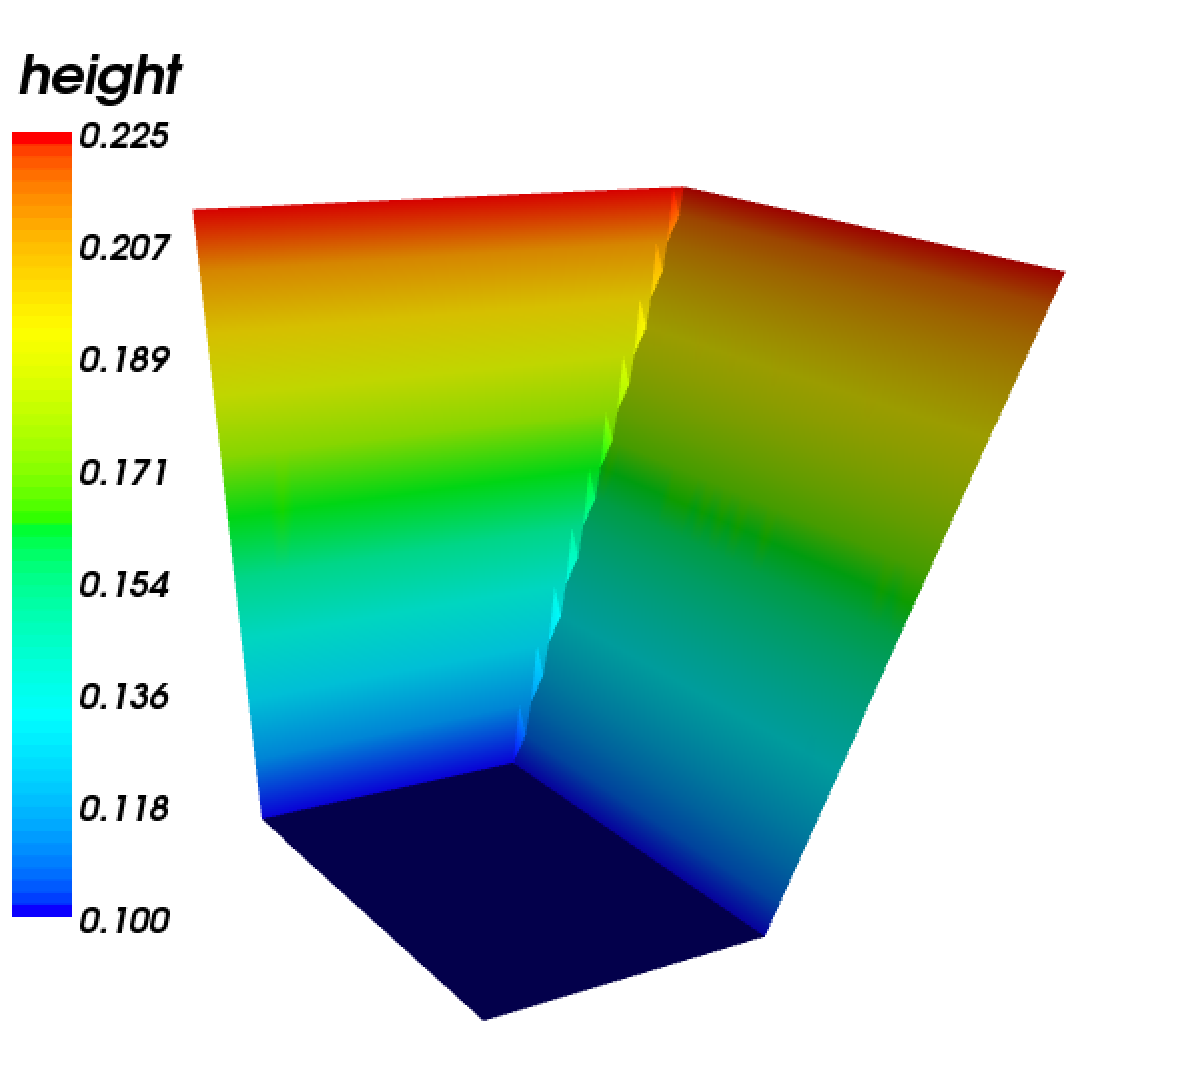
\includegraphics[width=\smallfig]{chapters/schroll/pdf/h0_typical.pdf}
    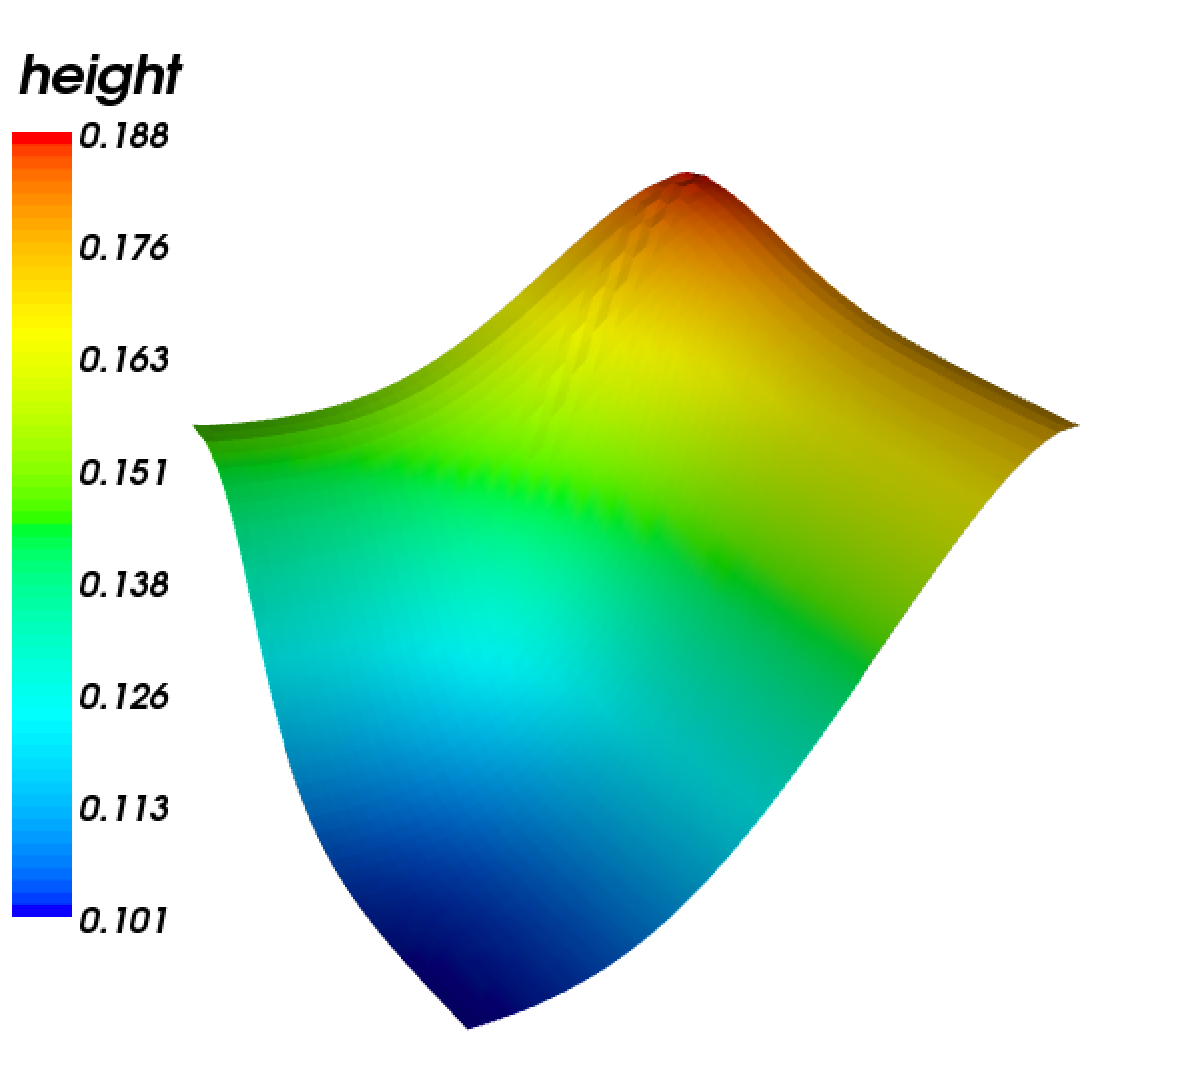
\includegraphics[width=\smallfig]{chapters/schroll/pdf/h_typical.pdf} \\
    \caption{Evolution of $h$, initial left, $t=0.04$ right.}
    \label{fig1}
  \end{center}
\end{figure}

To inspect the output functional, we generate synthetic data by
computing a reference solution.  In the first experiment, the
reference parameters are
$(\alpha_1, \alpha_2)=(\beta_1, \beta_2)=(0.8,0.8)$.  We fix $\beta$
to the reference values and scan the well output over the
$\alpha$-range $[0.0, 1.5]^2$. The upper left plot in
Figure~\ref{fig2} depicts contours of the apparently convex
functional, with the reference parameters as the global minimum.
Independent Landweber iterations, started in each corner of the domain
identify the optimal parameters in typically five steps.  The
iteration is stopped if $\| \nabla J(p^k) \| \le 10^{-7}$, an
indication that the minimum is reached.  In all figures below, a green
dot marks the optimal, calibrated parameters.  The lower left plot
shows the corresponding scan over $\beta$ where $\alpha=(0.8,0.8)$ is
fixed.  Obviously the search directions follow the steepest decent,
confirming that the gradients are correctly evaluated via the dual
solution.  In the right column of Figure~\ref{fig2} we see results for
the same experiments, but with 5\% random noise added to the synthetic
well data.  In this case the optimal parameters are of course not the
reference parameters, but still close.  The global picture appears
stable with respect to noise, suggesting that the concept allows to
calibrate diffusive, depositional models to data observed in wells.

\begin{figure}
  \begin{center}
    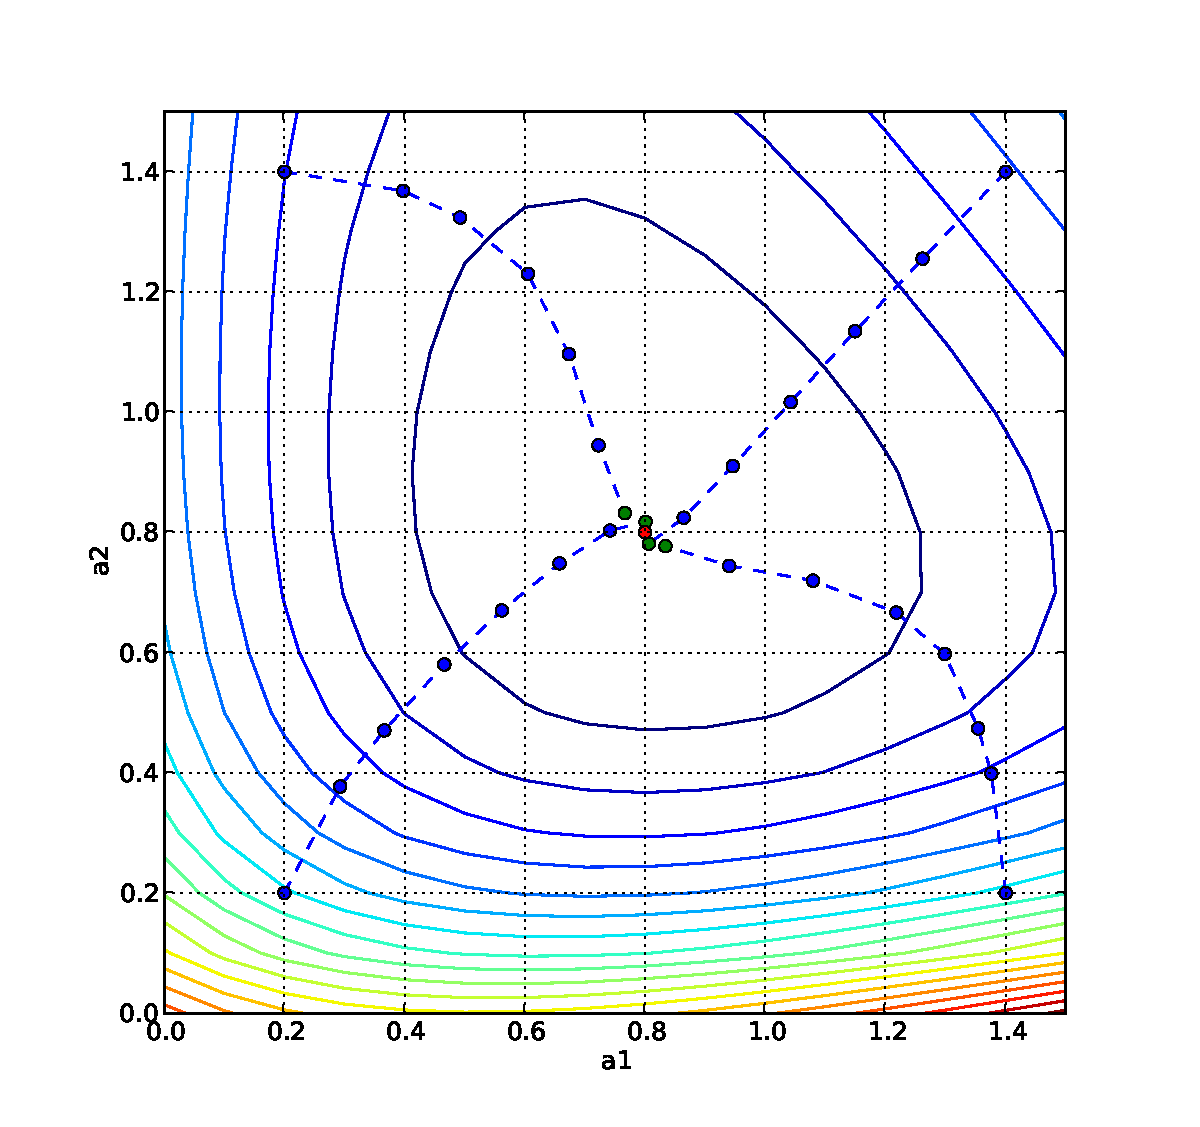
\includegraphics[width=\smallfig]{chapters/schroll/pdf/a1a2scan4.pdf}
    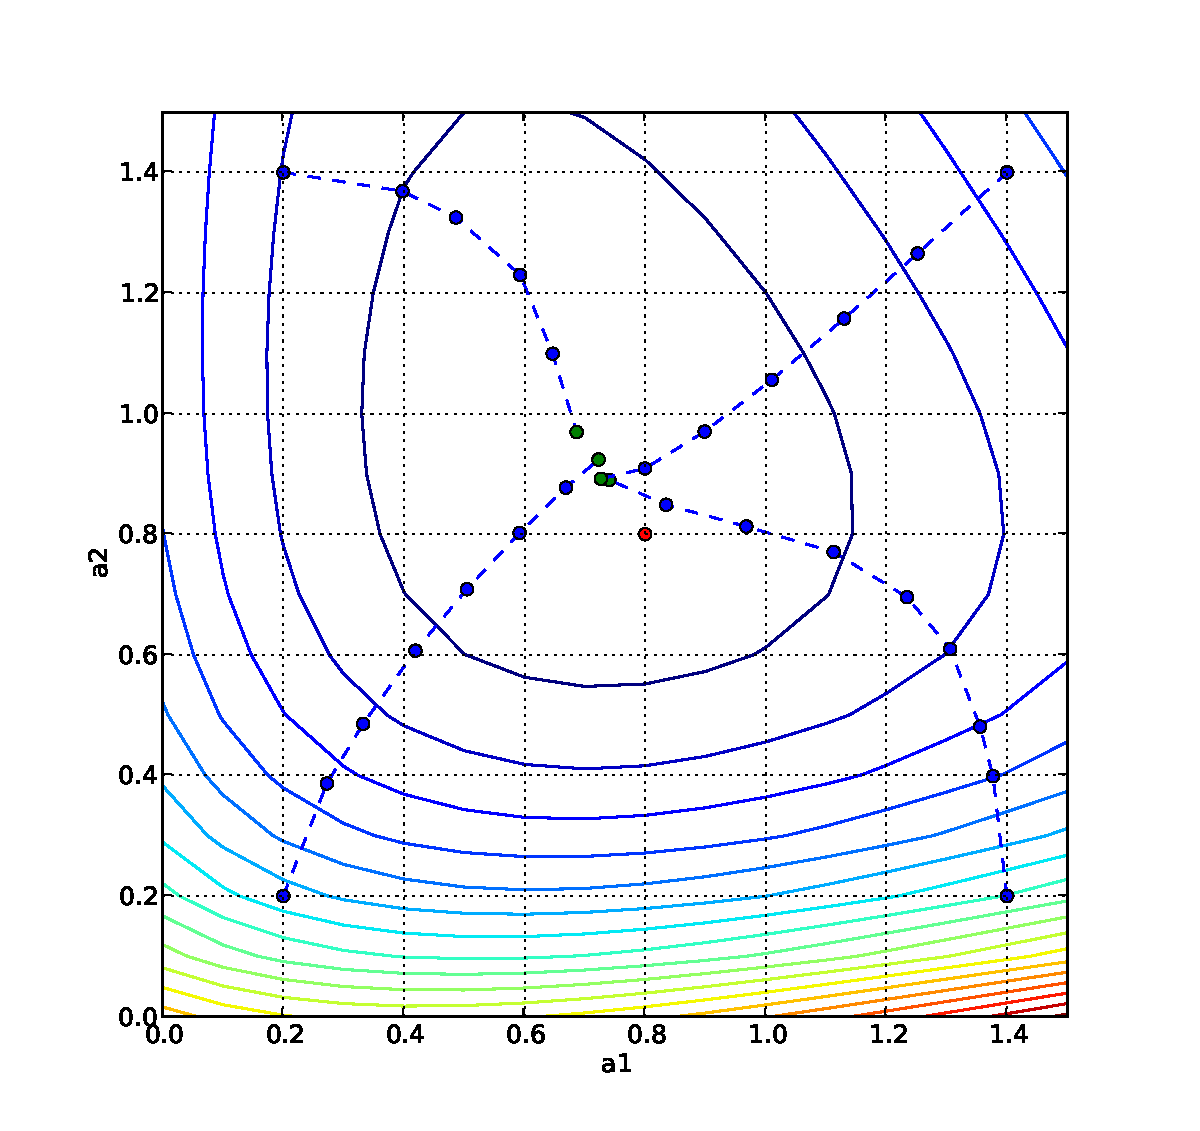
\includegraphics[width=\smallfig]{chapters/schroll/pdf/a1a2scan4-5.pdf}
    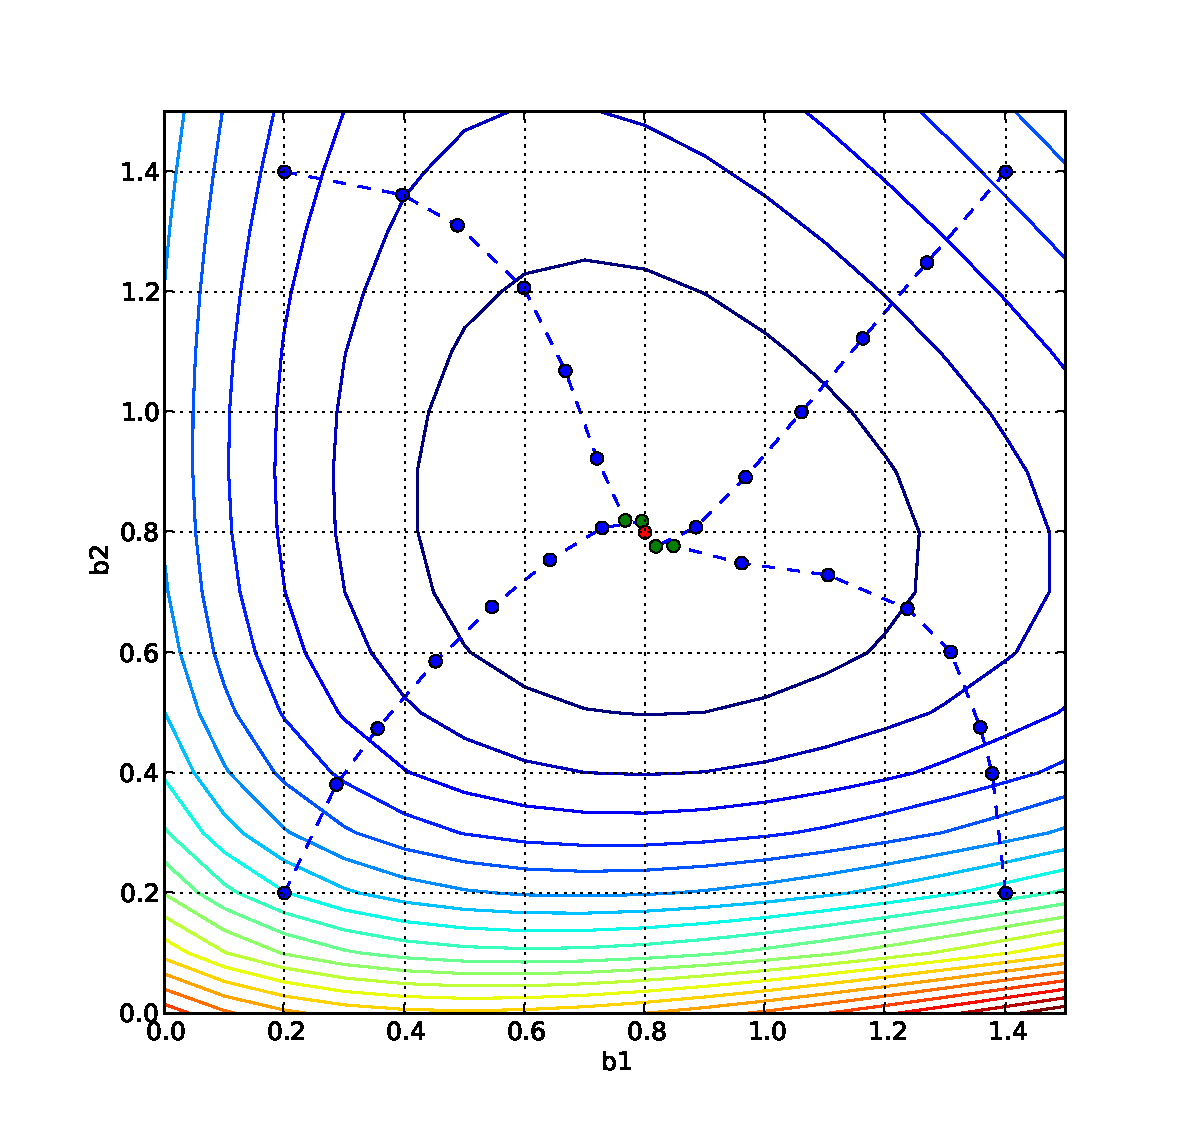
\includegraphics[width=\smallfig]{chapters/schroll/pdf/b1b2scan4.pdf}
    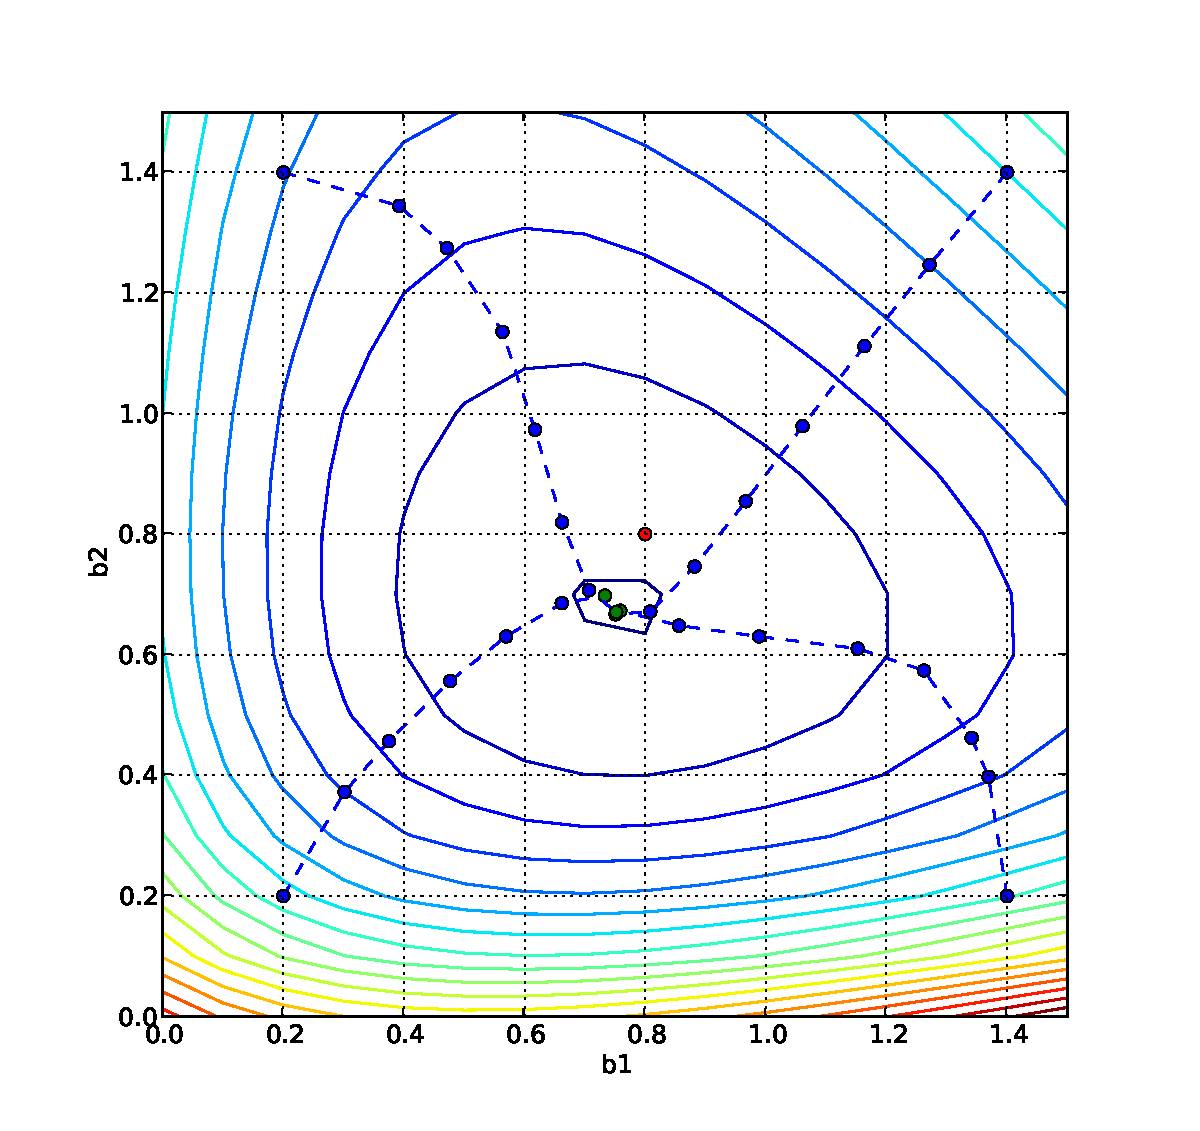
\includegraphics[width=\smallfig]{chapters/schroll/pdf/b1b2scan4-5.pdf}
    \caption{Contours of $J$ and Landweber iterations. Optimal parameters
    (green), reference parameters (red).
      Clean data left column, noisy data right. $\alpha$-iterations
      upper row, $\beta$-iterations lower row.}
    \label{fig2}
  \end{center}
\end{figure}

Ultimately, the goal is to calibrate all four parameters $\alpha =
(\alpha_1, \alpha_2)$ and $\beta = (\beta_1, \beta_2)$ to available
data.  Figure~\ref{fig3} depicts Landweber iterations in four
dimensional parameter space, started at $\alpha=(1.4, 0.2)$ and
$\beta=(0.2, 1.4)$.  Actually, projections onto the $\alpha$ and
$\beta$ coordinate plane are shown.  Obviously, both iterations
converge and, without noise added, the reference parameters, $\alpha
= \beta = (0.8, 0.8)$, are detected as optimal parameters.  Adding 5\%
random noise to the recorded data, we simulate data observed in wells.
In this situation, see the right column, the algorithm identifies
optimal parameters, which are clearly off the reference.
Fig.~\ref{fig7} depicts fifty realizations of this experiments.  The
distribution of the optimal parameters is shown together with their
average in red.  The left graph in Fig.~\ref{fig7} corresponds to the
reference parameters
$(\alpha_1, \alpha_2)=(\beta_1, \beta_2)=(0.8,0.8)$ as in
Fig.~\ref{fig3}.  On average the calibrated, optimal parameters are
$\bar\alpha=(0.860606, 0.800396)$ and $\bar\beta=(0.729657, 0.827728)$
with standard deviations $(0.184708, 0.127719)$ and $(0.176439,
0.12411)$.

\begin{figure}
  \begin{center}
    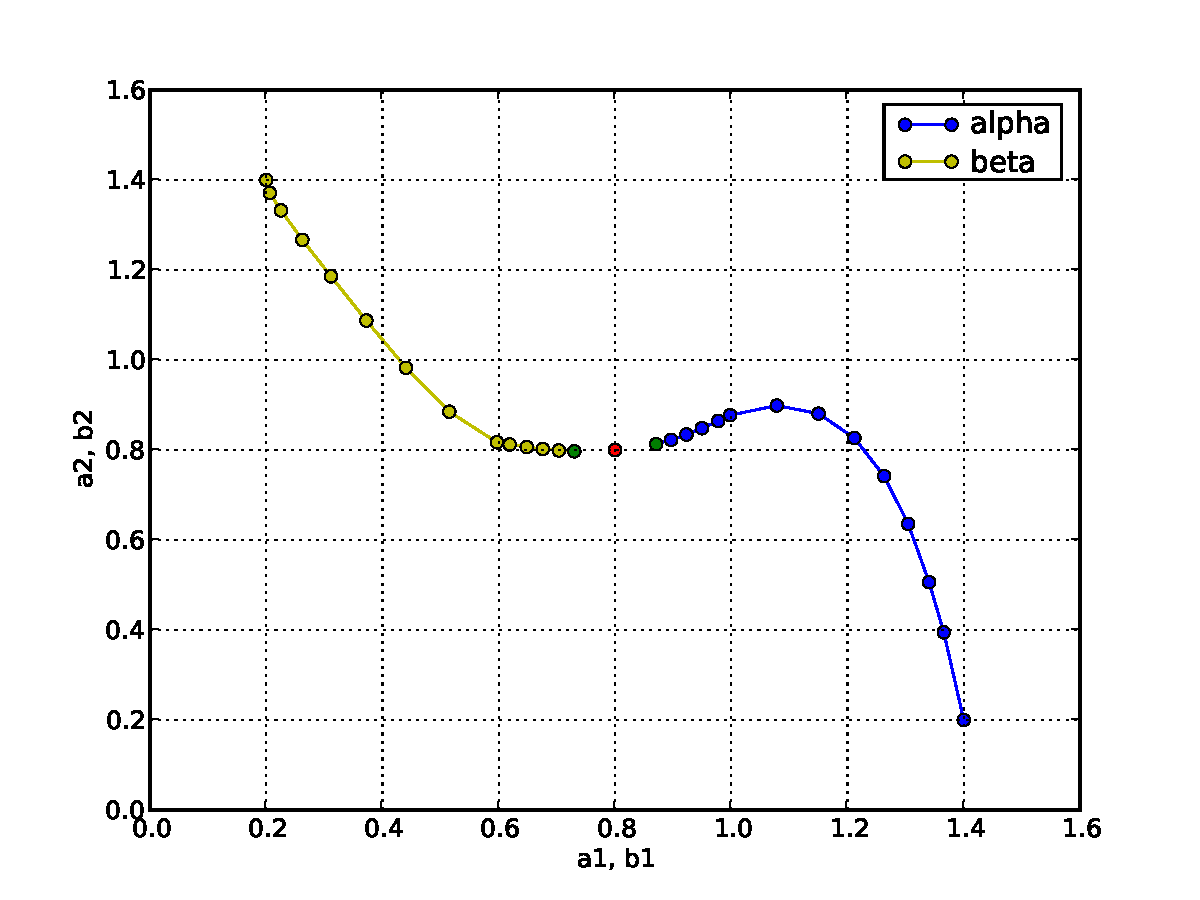
\includegraphics[width=\smallfig]{chapters/schroll/pdf/4Dscan3.pdf}
    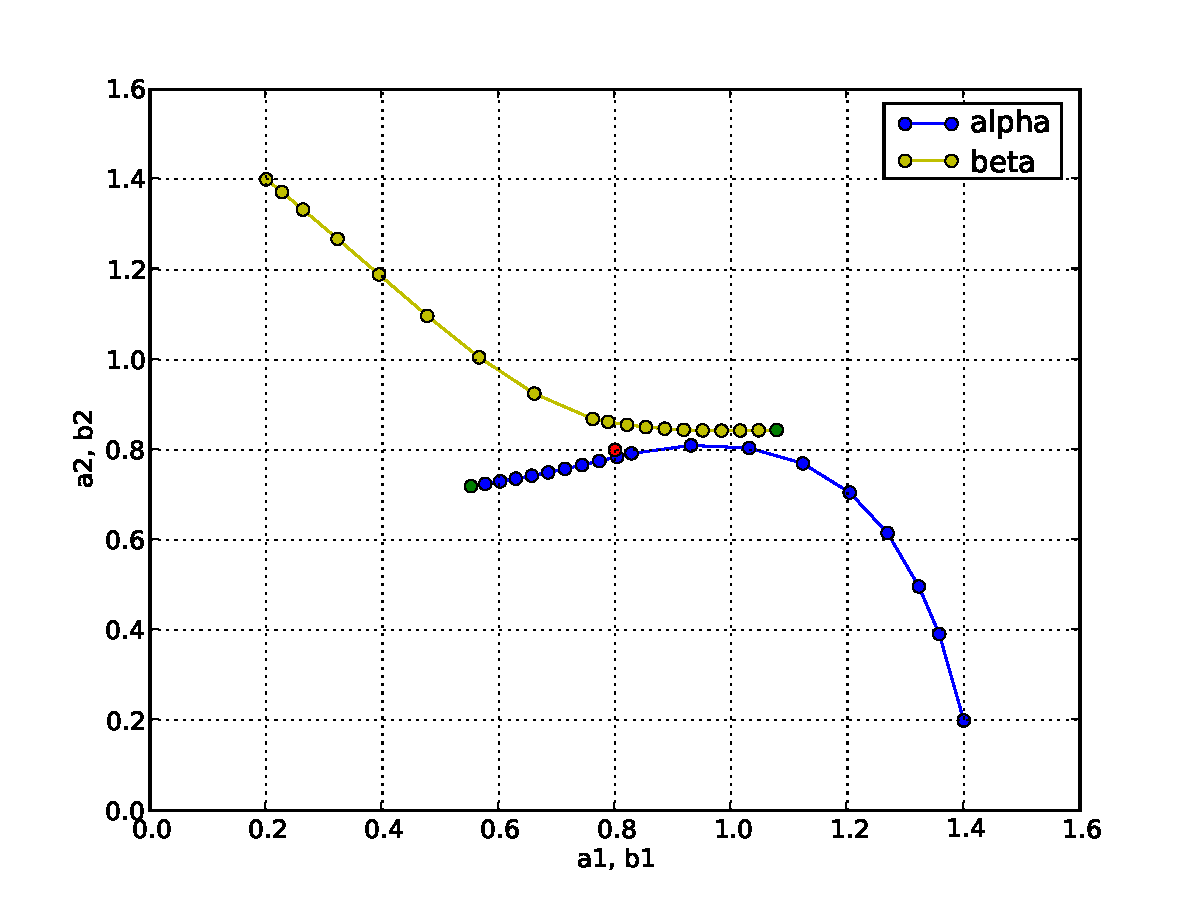
\includegraphics[width=\smallfig]{chapters/schroll/pdf/4Dscan3-5.pdf}
    \vspace{-0.7cm}
    \caption{Landweber iterations. Optimal parameters (green), reference
    parameters (red). Clean (left) and noisy data (right).}
    \label{fig3}
  \end{center}
\end{figure}

In the next experiments non uniform reference parameters are set for
$\alpha = (0.6, 1.0)$ and $\beta = (1.0, 0.6)$.  Figure~\ref{fig4}
shows iterations with the noise-free reference solution used as data
on the left hand side.  Within the precision of the stopping
criterion, the reference parameters are detected.  Adding 5\% noise to
the well data leads to different optimal parameters, just as expected.
On average however, the optimal parameters obtained in repeated
calibrations $\bar\alpha=(0.676051, 1.03604)$ and
$\bar\beta=(0.902532, 0.602344)$ match the reference parameters quite
well, see Figure~\ref{fig7}, right hand side.  The standard deviations
in this case are $(0.18374, 0.0886383)$ and $(0.166801, 0.0750035)$
respectively.

\begin{figure}
  \begin{center}
    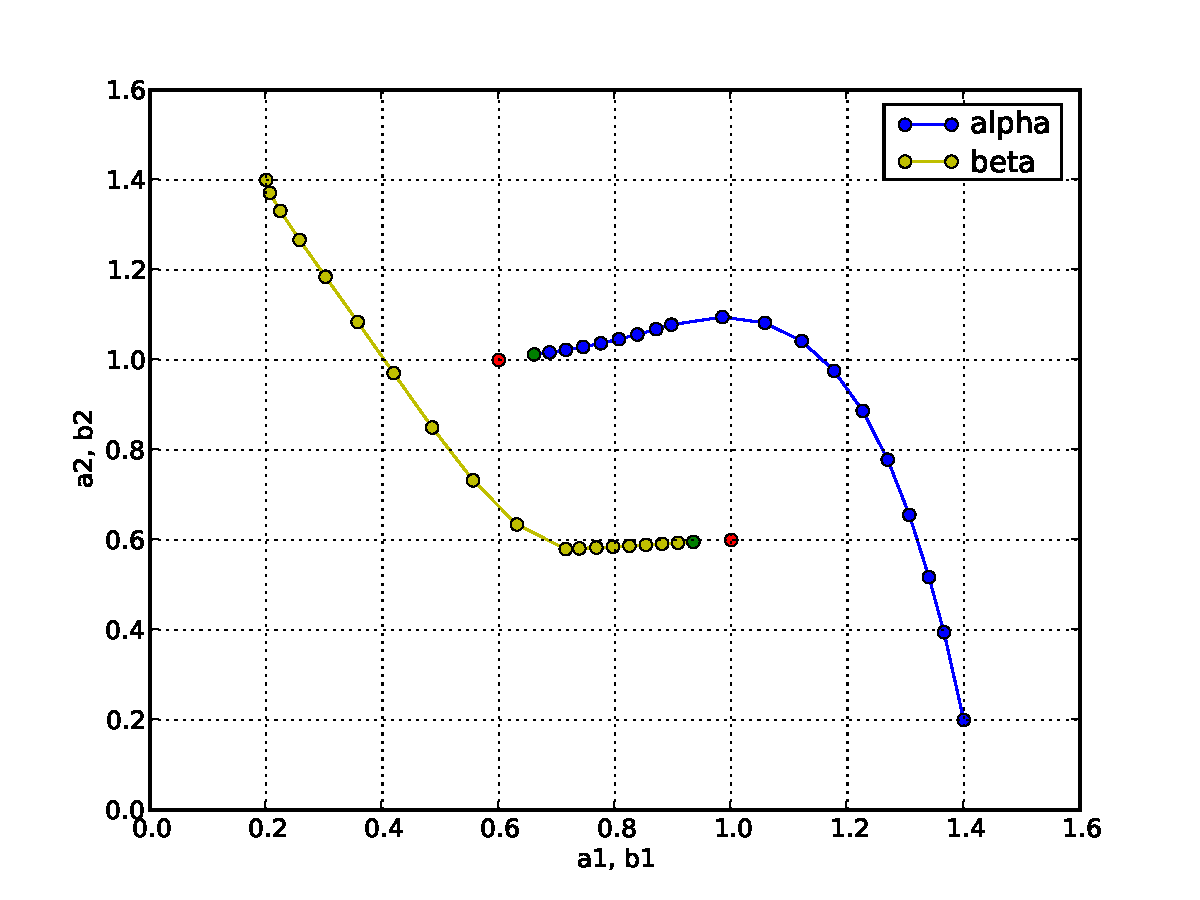
\includegraphics[width=\smallfig]{chapters/schroll/pdf/4Dscan3b.pdf}
    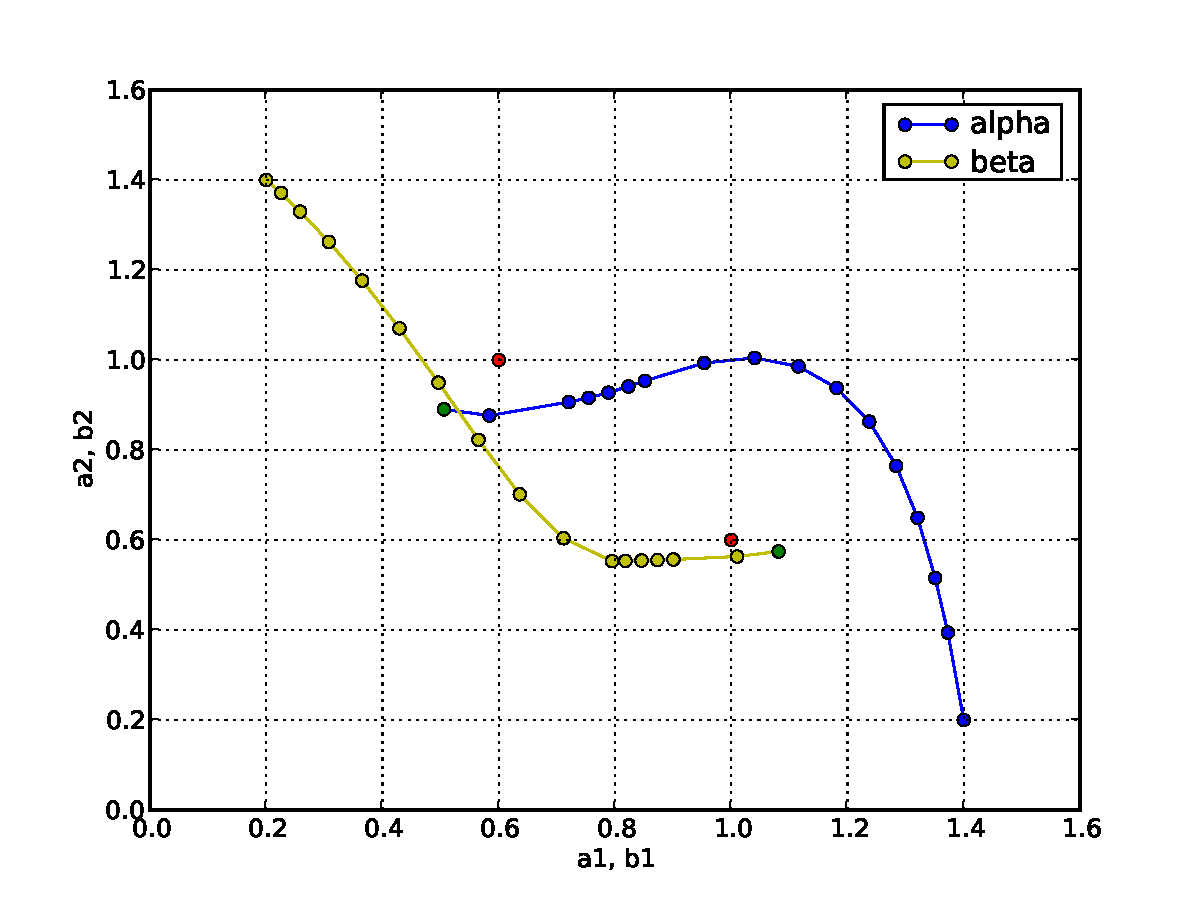
\includegraphics[width=\smallfig]{chapters/schroll/pdf/4Dscan3b-5.pdf}
    \vspace{-0.7cm}
    \label{fig4}
    \caption{Landweber iterations. Optimal parameters (green), reference
    parameters (red). Clean (left) and noisy data (right).}
  \end{center}
\end{figure}

\begin{figure}
  \begin{center}
    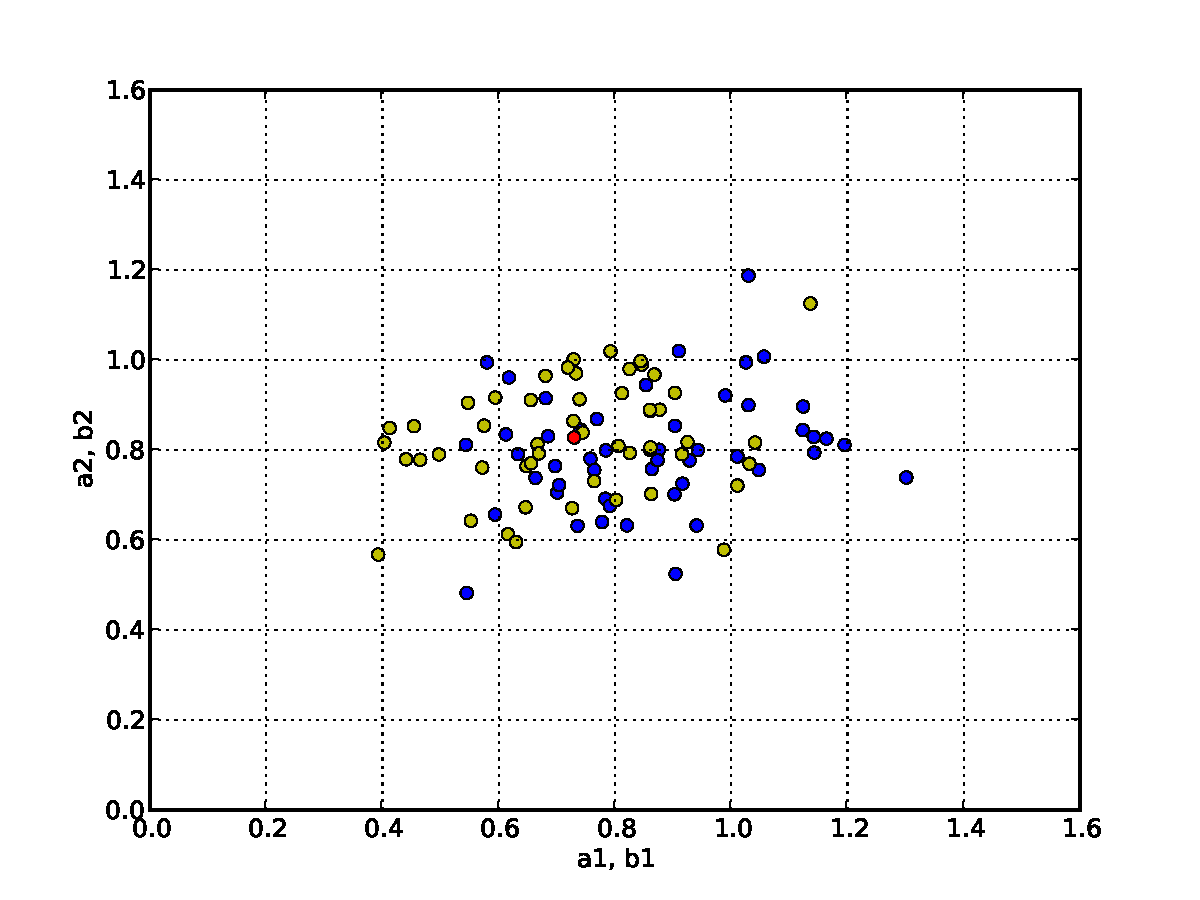
\includegraphics[width=\smallfig]{chapters/schroll/pdf/4Dsample3-5.pdf}
    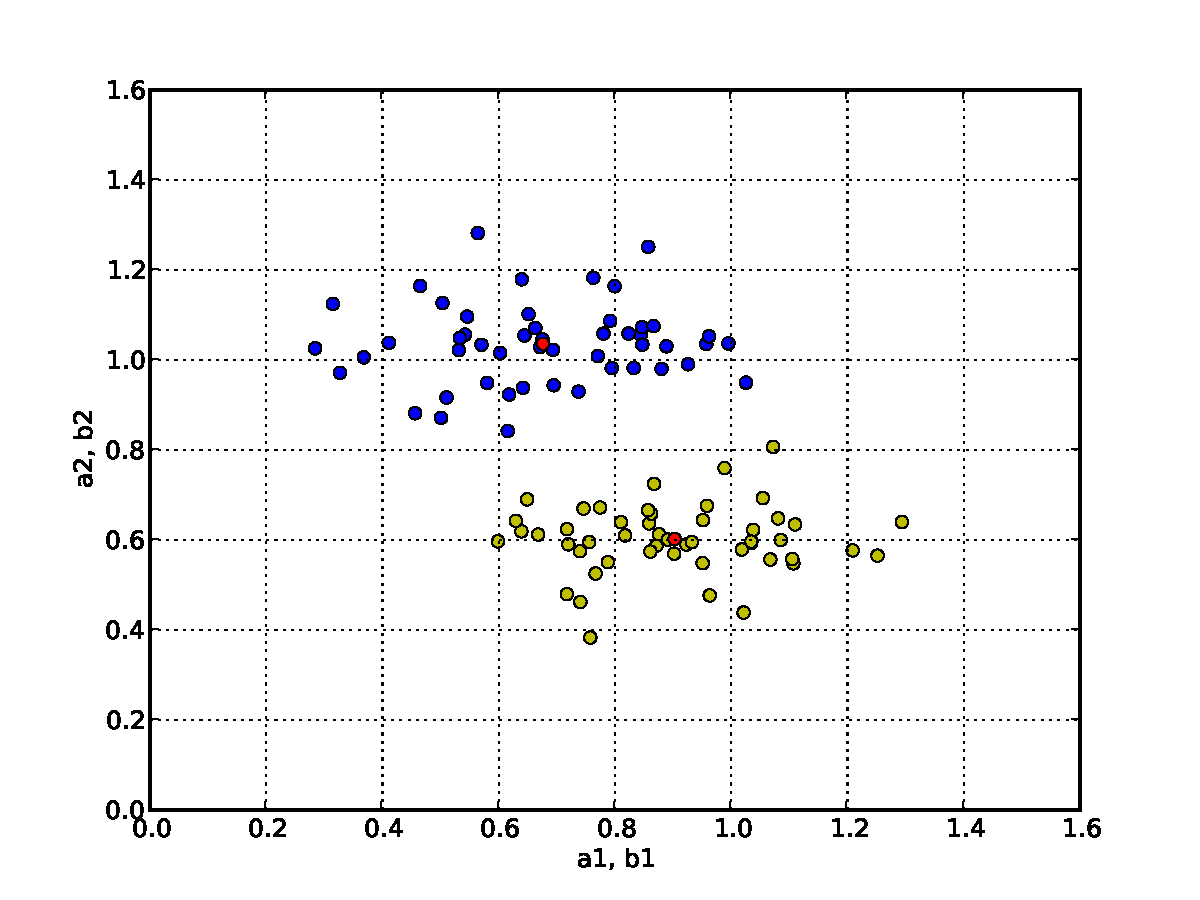
\includegraphics[width=\smallfig]{chapters/schroll/pdf/4Dsample3b-5.pdf}
    \vspace{-0.7cm}
    \caption{Sets of optimal parameters calibrated to noisy data, $\alpha$
    blue, $\beta$ yellow, average red.}
    \label{fig7}
  \end{center}
\end{figure}

In the last experiment, $\alpha$ is discontinuous along $x=1/2$, while
$\beta$ is discontinuous along $y=1/2$:
\begin{equation}
 \alpha = \left\{
 \begin{array}{rl} 1.0 & x \ge 1/2 \\[\jot] 0.6 & x < 1/2 \end{array}
 \right .
 , \quad
 \beta = \left\{
 \begin{array}{rl} 0.6 & y \ge 1/2 \\[\jot] 1.0 & y < 1/2 \end{array}
 \right .
 .
\end{equation}
In this way the evolution is governed by different diffusion parameters
in each quarter of the basin.
Having placed one well i each quarter,
one can effectively calibrate the model to synthetic data with and without random noise,
as shown in Figure~\ref{fig6}.

\begin{figure}
  \begin{center}
    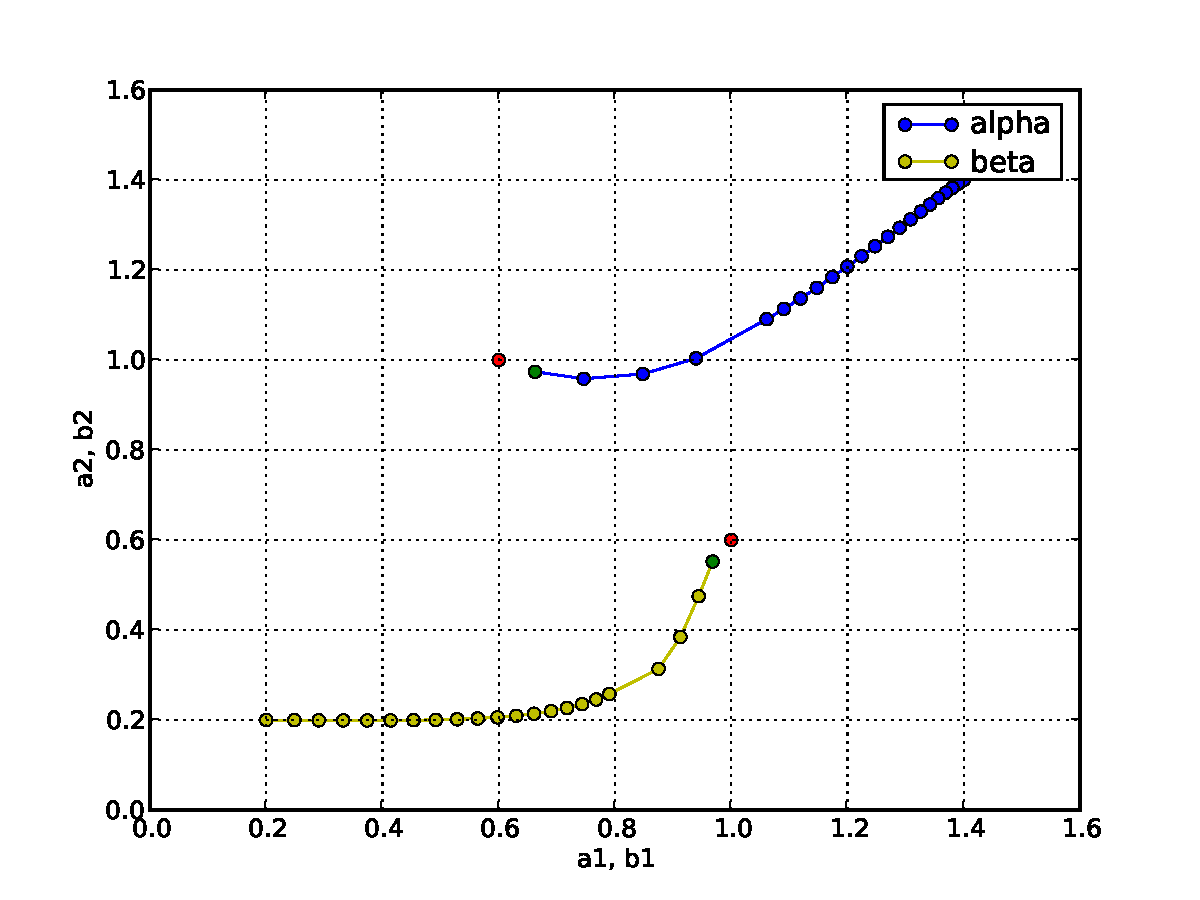
\includegraphics[width=\smallfig]{chapters/schroll/pdf/4D-1scan4b.pdf}
    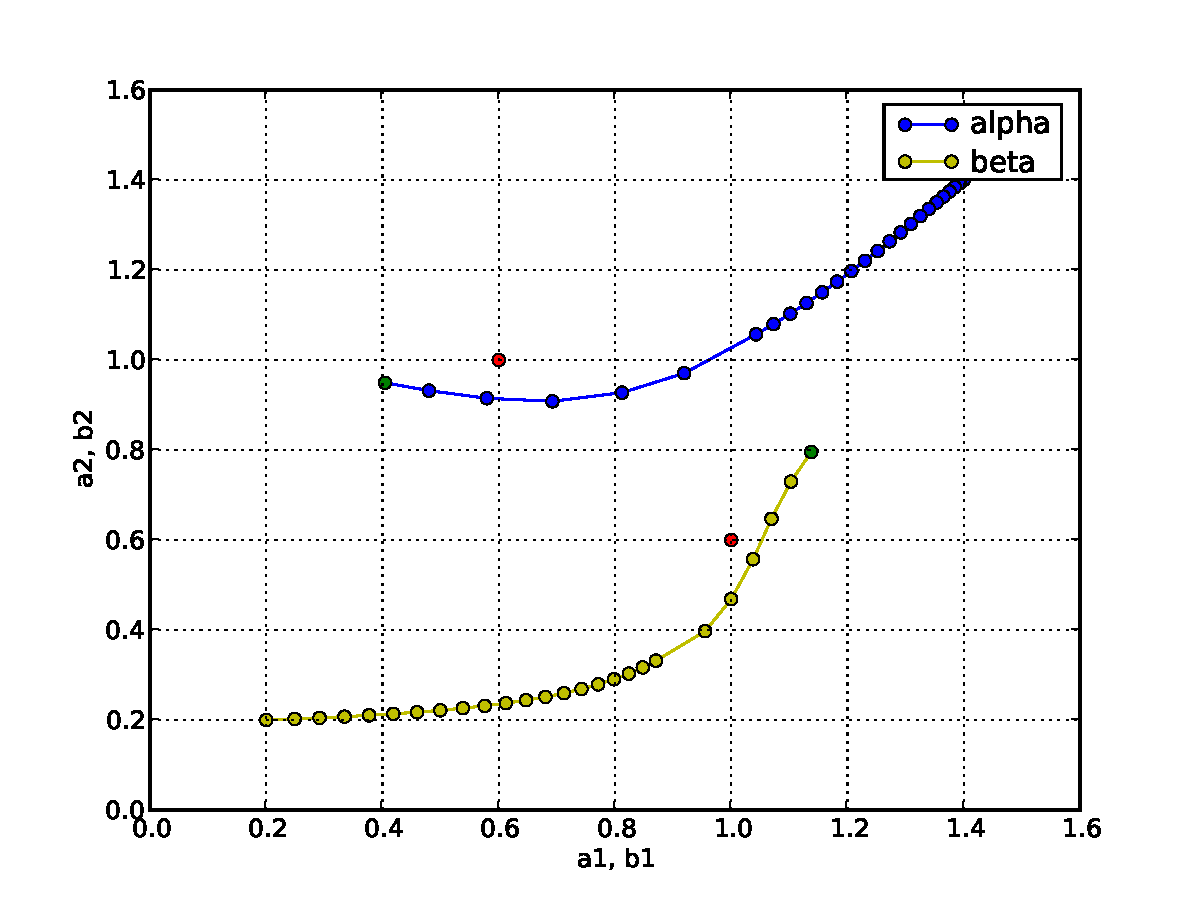
\includegraphics[width=\smallfig]{chapters/schroll/pdf/4D-1scan4b-5.pdf}
    \vspace{-0.7cm}
    \caption{Landweber iterations. Optimal parameters (green), reference
    parameters (red). Clean (left) and noisy data (right).}
    \label{fig6}
  \end{center}
\end{figure}

%------------------------------------------------------------------------------
\section{Results and conclusion}

The calibration of piecewise constant diffusion coefficients using
local data in a small number of wells is a well behaved inverse
problem.  The convexity of the output functional, which is the basis
for a successful minimization, remains stable with random noise added
to the well data.  The Landweber algorithm, with duality based
gradients, automatically detects optimal parameters.  As the dual
problems are derived in variational form, the FEniCS project DOLFIN is
the ideal tool for efficient implementation.

\subsection*{Acknowledgements}

The author wants to thank Are Magnus Bruaset for initiating this work.
Many thanks to Bj{\o}rn Fredrik Nielsen for thoughtful suggestions
regarding inverse problems as well as Anders Logg and Ola Skavhaug for
their support regarding the DOLFIN software.

The presented work was funded by a research grant from Statoil.  The
work has been conducted at Simula Research Laboratory as part of CBC,
a Center of Excellence awarded by the Norwegian Research Council.



